\section{Relational Databases}

\subsection{SQL and First-Order Logic}

\todo{figures + explain binary relations (nice figures) and $\atom{a}$ notation.}

The most common model of databases is by far that of "relational databases",
in which data is stored in \emph{tables}: an example is depicted
in \Cref{fig:relational-database-cinema}.

\begin{table}
	\centering%
	{%
	\footnotesize%
	\begin{tabular}{cccc}
		\multicolumn{4}{c}{\textsc{Movies}} \\ \toprule
		id & title & length & director \\ \midrule
		197 & Eyes Wide Shut & 159 & Stanley Kubrick \\ 
		205 & J'ai tué ma mère & 96 & Xavier Dolan \\
		304 & Amadeus & 161 & Miloš Forman \\
		321 & 120 Battements par minute & 143 & Robin Campillo \\ \bottomrule
	\end{tabular}
	\\\bigskip%
	\begin{tabular}{cc}
		\multicolumn{2}{c}{\textsc{Rooms}} \\ \toprule
		id & capacity  \\ \midrule
		1 & 108 \\
		2 & 124 \\
		3 & 96 \\
		4 & 102 \\ \bottomrule
	\end{tabular}%
	\hspace{1cm}%
	\begin{tabular}{ccc}
		\multicolumn{3}{c}{\textsc{Projections}} \\ \toprule
		movie\_id & room\_id & time \\ \midrule
		197 & 2 & 2025-03-28 14:00 \\
		205 & 3 & 2025-03-28 14:30 \\
		321 & 4 & 2025-03-28 14:30 \\
		197 & 1 & 2025-03-28 17:00 \\ \bottomrule
	\end{tabular}
}
	\caption{
		\AP\label{fig:relational-database-cinema}
		A "relational database" consisting of three tables, representing data
		stored by a cinema. (Replica of \Cref{fig:example-db-as-rel}.)
	}
\end{table}

Formally, a \AP""pointed relational database"" $\tup{\?D, \bar d}$
over a "purely relational signature" $\sigma$
consists of, for each "predicate" $\+R$ of arity $k$ in $\sigma$,
a $k$-ary relation $\+R_{(k)}(\?D)$, as well as a tuple $\bar d$ of elements.%
A \AP""relational database"" is a "pointed relational database" whose tuple is empty.
\footnote{It is often asked that at least one $\+R_{(k)}(\?D)$ is non-empty.
Whether this condition is imposed does change the theory---for instance the "first-order sentences"
that are valid over all non-empty structures is a strict subset of
those valid over all (possible empty) structures.
However, this condition is mostly required for historical reasons,
and whether the databases are allowed to be non-empty
will be of little importance for the query languages we will consider.}
Each tuple of some relation $\+R_{(k)}(\?D)$ is called a \emph{fact}.
From a practical perspective, relations model the tables,
while each fact correspond to some row: for 
instance the database of \Cref{fig:relational-database-cinema}
has three relations, twelve facts and no constants.%
\footnote{Many variations on the definition above exists:
for instance the columns of the table are often given a name (called \emph{attribute}),
see "eg" \cite[\S\!\S~3.1--3.2]{AbiteboulHullVianu1995Databases}.
This is usually done to make the syntax of relational algebra for readable,
however this is only syntactic sugar \cite[Proposition~5.1.2]{AbiteboulHullVianu1995Databases}.}

Naturally, each "relational database" yields a "$\sigma$-structure" whose
domain is the set of elements occurring in some fact of the database or in the tuple.
This structure has the property that each vertex belongs to some "hyperedge" or
is a constant: in other words, it has no \AP""isolated vertices"".
This mapping is in fact one-to-one: "relational databases" over $\sigma$
are in bijection with "$\sigma$-structures" with no "isolated vertices".

\begin{hypothesisnotation}
	We identify (pointed) "relational databases" with (pointed) "relational structures"
	with no "isolated vertices".
\end{hypothesisnotation}

As mentioned in \Cref{ch:intro}, from a theoretical perspective,
a very natural way of querying these "structures"
is "via" "first-order logic". Remarkably, it is exactly as expressive 
as the fragment of SQL consisting of queries generated by
\begin{align}
	\phi_{(k)}\; & \mathrel{{:}{:}{=}} \sqlop{SELECT DISTINCT} \textrm{ attribute}_1, \dotsc, \textrm{ attribute}_k\notag\\
	& \hphantom{\mathrel{{:}{:}{=}}} \sqlop{FROM } \phi_{(i_1)}, \dotsc, \phi_{(i_n)}\notag\\
	& \hphantom{\mathrel{{:}{:}{=}}} \sqlop{WHERE} \textrm{ some condition} \label{eq:sql-fo}\\
	& \;\mid \textrm{some table of arity $k$} \notag\\
	& \;\mid \phi_{(k)} \mathrel{\sqlop{ UNION }} \phi_{(k)}
		\mid \phi_{(k)} \mathrel{\sqlop{ EXCEPT }} \phi_{(k)}
		\mid \phi_{(k)} \mathrel{\sqlop{ INTERSECT }} \phi_{(k)}, \notag
\end{align}
where $i_1 + \dotsc + i_n = k$ and the condition after $\sqlop{WHERE}$
is a conjunction of equalities between attributes.
Dealing with the arity $k \in \N$ is required to ensure "eg" that the union 
is homogeneous---"ie" that all facts in the union have the same arity.%
\footnote{Also, the \textsf{DISTINCT} keyword is only necessary because SQL
has a multiset semantics rather than a set-based semantics…}

\begin{proposition}[Codd's theorem {\cite[\S~4]{Codd1972RelationalCompleteness}}]
	\!\footnote{Codd's theorem actually deals
	with \emph{relational algebra} rather than SQL.
	The equivalence between \emph{relational algebra} and the fragment
	\eqref{eq:sql-fo} of SQL is however straightforward.
	See also \cite[Theorem~5.4.6]{AbiteboulHullVianu1995Databases}.}
	\AP\label{prop:codd-thm}
	"First-order logic" over "$\sigma$-structures" with no "isolated vertices"
	is equally expressive to the SQL fragment defined in \eqref{eq:sql-fo}.
	Moreover, this equivalence is effective.
\end{proposition}

\begin{proof}[Proof sketch]
	\emph{Warning:} dealing with all the subtleties of the proof is actually
	somewhat tedious. Hence, we provide an \emph{informal} proof,
	which prioritizes intuition over formalism.

	Expressing a SQL query as a "first-order formula" is intuitive,
	by generalizing the idea given in \Cref{sec:intro-cq}:
	\begin{itemize}
		\item $\sqlop{UNION}$, $\sqlop{EXCEPT}$ AND $\sqlop{INTERSECT}$
			are interpreted as the union, set difference ("ie" $- \land (\neg -)$)
			and intersection;
		\item a table of arity $k$, modelled as a relation $\+R_{(k)}$,
			is encoded as the atomic formula
			\[
				\phi_{(k)}(x_1,\hdots,x_k) \defeq \+R_{(k)}(x_1,\hdots,x_k)
			\]
			with $k$ free variables which are all fresh;
		\item a query
			\begin{align*}
				& \sqlop{SELECT DISTINCT} \textrm{ attribute}_1, \dotsc, \textrm{ attribute}_k \\
				& \sqlop{FROM } \phi^1_{(i_1)}, \dotsc, \phi^n_{(i_n)} \\
				& \sqlop{WHERE} \theta 
			\end{align*}
			is encoded as
			\[
				\psi(y_1,\hdots,y_k) \defeq
				\exists \bar x.\;
				\phi^1_{(i_1)}(x^1_1,\dotsc,x^1_{i_1})
				\land \dotsc \land
				\phi^n_{(i_n)}(x^n_1,\dotsc,x^n_{i_n})
				\land \theta,
			\]
			with $y_1$, $\dotsc$, $y_k$ being the variable associated
			to the attributes---"eg" if $\textrm{attribute}_1$ is the
			third attribute of $\phi^2$, then $y_1 \defeq x^2_3$---
			and $\bar x$ is the tuple of all variables of the form $x^i_j$
			that are distinct from the $y_i$'s.
	\end{itemize}
	
	The converse encoding, "ie" from first-order logic to SQL queries,
	is a little more tricky:
	\begin{itemize}
		\item union is encoded with \sqlop{UNION},
			intersection and existential quantification with
			\sqlop{SELECT DISTINCT}-\sqlop{FROM}-\sqlop{WHERE};
		\item we encode negation using \sqlop{EXCEPT} and a SQL query
			that outputs every $k$-tuple of vertices of the "structure"---this query can
			be written as a big union of \sqlop{SELECT DISTINCT}-\sqlop{FROM}
			queries;
		\item lastly, universal quantification can then be obtained
			using the tautology
			\[\forall x.\; \phi(x) \equiv \neg\exists x.\; \neg \phi(x).\qedhere\]
	\end{itemize}
\end{proof}

A crucial ingredient that ensures the correctness of these encodings
is actually the fact that "relational databases" are encoded
as "relational structures" \textbf{with no "isolated variables"}.%
\footnote{The restriction of "first-order logic" to
"relational databases" is usually called \emph{relational calculus}.}
Take for instance the "first-order formula"
$\neg \textsc{Room}(x,y)$:
we expressed it in SQL as
\[
	\textrm{All pairs}
	\mathrel{\sqlop{ EXCEPT }}
	(\sqlop{SELECT DISTINCT } x, y \mathrel{\sqlop{ FROM }} \textsc{Room})\; 
\]
where `All pairs' is a query outputting all pairs in the database.
The equivalence, or more precisely the fact that the semantics
of the "first-order formula" over the "relational structure"
is included in the semantics of the SQL query over the "relational structure", is
precisely permitted by the lack of "isolated vertices" in
the "structure": for more details, we refer the reader 
to the term ``active domain'' in \cite{AbiteboulHullVianu1995Databases}.%
\footnote{The same query is actually a good example of why there is no built-in
negation in SQL, even though it would not change its expressiveness: it
is actually very hard to image a situation where
knowing that `Xavier Dolan' is not the id of a room with capacity `2025-03-28 14:00'
would be useful…}

The expressiveness of this fragment of SQL however comes to the cost
of computational efficiency.

\begin{proposition}[Folklore]
	Given a "first-order formula" $\phi(\bar x)$, a "relational structure" $\?D$
	with no "isolated vertices", and a tuple $\bar d$, deciding
	if $\bar d \in \semFO{\phi(\bar x)}{\?D}$
	is "PSpace"-complete.
\end{proposition}

\begin{proof}[Proof sketch]
	The upper bound can be proven by considering the naïve algorithm
	that recurses on the formula.
	The lower bound follows from a trivial reduction from
	the "quantified Boolean formula problem".
\end{proof}

Even worth, when turning to the \emph{static analysis} of these queries, 
the problems become undecidable. Given two (semantical) "queries" $\phi$ and $\psi$,
we say that they are "semantically equivalent"---implicitly
over "finite@@struct" "relational databases"---when for every "finite@@struct" "relational databases" $\?D$, we have $\?D \in \phi$ "iff" $\?D \in \phi'$.
This fact is denoted by \AP$\phi \intro*\semequiv \phi'$.

\begin{proposition}[Trakhtenbrot $\ast$ Databases, see "eg" {\cite[Theorem~6.3.1 \& Corollary~6.3.2]{AbiteboulHullVianu1995Databases}}]
	\!\footnote{This result is often incorrectly confused with
	"Trakhtenbrot's theorem", which deals with all "relational structures".
	However, the notion of "semantical equivalence" differs when considered
	over "relational databases" or all "relational structures".}
	\AP\label{prop:Trakhtenbrot-db}
	It is undecidable whether a
	"first-order formula" is satisfiable over finite "relational databases".
	In turn, validity and "semantical equivalence" are also undecidable.
\end{proposition}

In turn, it means that there is no hope to optimize a SQL query from the
fragment \eqref{eq:sql-fo}, in the sense of \Cref{sec:intro-existential}.%

\begin{corollary}[Folklore than is unfortunately often not mentionned, see "eg"
	{\cite[Remark~5.3]{AdlerWeyer2012TreeWidthFirstOrder}}]
	\label{coro:undecidability-minimization}
	Given a "first-order formula" $\phi$ and $k\in\N$, it is undecidable
	whether $\phi$ is "semantically equivalent" to a "formula@@FO" with at most $k$ variables.
\end{corollary}

\subsection{Conjunctive Queries to the Rescue}

The undecidability results of \Cref{prop:Trakhtenbrot-db,coro:undecidability-minimization},
together with the fact that queries occurring in practice---see \Cref{sec:intro-cq}---are
much simpler than the formulas occurring in the undecidability proof motivate
the study of well-behaved query fragments.

"Conjunctive queries" arise as either the fragment
\begin{align}
	\phi_{(k)}\; & \mathrel{{:}{:}{=}} \sqlop{SELECT DISTINCT} \textrm{ attribute}_1, \dotsc, \textrm{ attribute}_k\notag\\
	& \hphantom{\mathrel{{:}{:}{=}}} \sqlop{FROM } \phi_{(i_1)}, \dotsc, \phi_{(i_n)}\label{eq:sql-cq}\\
	& \hphantom{\mathrel{{:}{:}{=}}} \sqlop{WHERE} \textrm{ some condition} \notag\\
	& \;\mid \textrm{some table of arity $k$} \notag
\end{align}
of SQL, where, once again, $i_1 + \dotsc + i_n = k$ and the condition after $\sqlop{WHERE}$
is a conjunction of equalities between attributes.
From the proof of \Cref{prop:codd-thm} it actually follows that this fragment is exactly
as expressive as the fragment of "first-order logic", restricted to "relational databases",
generated by 
\begin{align}
	\phi \mathrel{{:}{:}{=}} \+R_{(k)}(x_1,\dotsc,x_k) \mid \phi \land \phi \mid \exists x.\; \phi,
	\label{eq:fo-cq}
\end{align}
where $\+R_{(k)}$ ranges over the "signature".

Now observe that, when dealing with the fragment \eqref{eq:fo-cq},
the "first-order formula" $(\exists x.\; \phi(x, \bar y)) \land \psi(\bar z)$
is equivalent to $\exists x'.\; (\phi(x', \bar y) \land \psi(\bar z))$
where $x'$ is any variable that occurs neither in $\bar y$ nor in $\bar z$.
For instance, we have 
\[
	(\exists x.\, \+P(x)) \land (\exists x.\, \exists y.\,\+R(x,y))
	\semequiv
	\exists z.\,\exists x.\, \exists y.\, \+P(z) \land \+R(x,y).
\]
This leads to a simple rewriting system that puts every formula from 
\eqref{eq:fo-cq} in so-called "prenex form".

\begin{proposition}[""Prenex form""]
	\AP\label{prop:prenex-form}
	Every formula from \eqref{eq:fo-cq} can be written in the form
	\begin{align}
		\exists \bar x.\, \bigwedge_{i=1}^n \+R^i_{(k_i)}(y^i_1,\dotsc,y^i_{k_i}).
		\label{eq:prenex-fo}
	\end{align}
\end{proposition}

\Cref{prop:prenex-form} has remarkable consequences.
Translating back the "formulas@@FO" in "prenex form" to 
SQL queries, it implies that the fragment \eqref{eq:sql-cq}
is no more expressive than its induction-free fragment
\begin{align}
	\phi_{(k)}\; & \mathrel{{:}{:}{=}} \sqlop{SELECT DISTINCT} \textrm{ attribute}_1, \dotsc, \textrm{ attribute}_k\notag\\
	& \hphantom{\mathrel{{:}{:}{=}}} \sqlop{FROM } \textrm{table}_{(i_1)}, \dotsc, \textrm{table}_{(i_n)}\label{eq:sql-cq-bis}\\
	& \hphantom{\mathrel{{:}{:}{=}}} \sqlop{WHERE} \textrm{ some condition}. \notag
\end{align}

Formally, we define a \AP"conjunctive query" to be
any "first-order formula" in "prenex form"---see \Cref{eq:prenex-fo}.
Recall that, as mentioned in \Cref{rk:prelim-formula-tuple},
we assume that "formulas" comes with a tuple of variables,
containing all free variables, potentially with repetition.
Hence, a \AP""conjunctive query"" over a "purely relational signature" $\sigma$,
or \reintro{CQ} for short, amounts to a finite set
of atomic formulas of the form $\+R_{(k)}(x_1,\hdots,x_k)$,
called ""atoms@@cq"", with $\+R_{(k)} \in \sigma$,
together with tuple of variables $\bar x$, called ""free variables@@cq""
or ""output variables@@cq"". The set of atoms is denoted conjunctively.
So, an example of "conjunctive query" is
\begin{align*}
	\gamma(\textsf{title}, \textsf{time}) \defeq\; 
	& \textsc{Movies}(\textsf{movie\_id}, \textsf{title}, \textsf{length}, \textsf{director}) \\
	& \land
	\textsc{Projections}(\textsf{movie\_id}, \textsf{room\_id}, \textsf{time}).
\end{align*} 
Semantically, it is interpreted as the "first-order formula" in "prenex form"
in which every variable that is not an "output variable" is quantified existentially,
giving in our case
\begin{align*}
	\gamma(\textsf{title}, \textsf{time}) \defeq\; 
	& \exists \textsf{movie\_id}.\, 
	\exists \textsf{length}.\, 
	\exists \textsf{director}.\,
	\exists \textsf{room\_id}.\, \\
	& \hphantom{\land~} \textsc{Movies}(\textsf{movie\_id}, \textsf{title}, \textsf{length}, \textsf{director}) \\
	& \land
	\textsc{Projections}(\textsf{movie\_id}, \textsf{room\_id}, \textsf{time}).
\end{align*} 

Interestingly, the semantics of "conjunctive queries" can be described using "homomorphisms",
via the theory of \emph{duality}.
\begin{definition}
	The "canonical database" associated to a "conjunctive query"
	\[
		\gamma(\bar x) = \bigwedge_{i=1}^n \+R^i_{(k_i)}(y^i_1,\dotsc,y^i_{k_i})
	\]
	over the "purely relational signature" $\sigma$ is the "pointed relational database"
	over $\sigma$ with tuple $\bar x$ and whose facts are
	$\+R^i_{(k_i)}(y^i_1,\dotsc,y^i_{k_i})$ for $i \in \intInt{1,n}$.
\end{definition}
We say that a "conjunctive query" is ""Boolean@@cq"" when it has no "output variables".
In this case, its "canonical database" is not only a "pointed relational database" but
in fact a "relational database".

\begin{proposition}[""Duality""]
	\AP\label{prop:duality}
	Let $\gamma(\bar x)$ be a "conjunctive query",
	and let $\tup{\?G, \bar x}$ denote its "canonical database".%
	\footnote{We denote the "canonical database" using the Roman
	uppercase associated with the Greek letter used to denote
	the query.}
	For any "pointed relational database" $\tup{\?D, \bar d}$,
	we have
	\[
		\bar d \in \semFO{\gamma(\bar x)}{\?D}
		\qquad\text{"iff"}\qquad
		\tup{\?G, \bar x} \homto \tup{\?D, \bar d}.
	\]
\end{proposition}

\begin{proof}
	This follows from the definition of "homomorphisms" and
	the semantics of "first-order logic".
\end{proof}

Duality has \emph{many} consequences. First, the following evaluation problem
lies in "NP", as it can be encoded into a "homomorphism problem".
\decisionproblem{""Conjunctive Query Evaluation""}{
	A "signature" $\sigma$,
	a "conjunctive query" $\gamma(\bar x)$ over $\sigma$,
	and a "pointed relational $\sigma$-database" $\tup{\?D, \bar d}$.
}{
	Does $\bar d \in \semFO{\gamma(\bar x)}{\?D}$?
}
For "Boolean conjunctive queries", both tuples are empty, and so
this amounts to asking whether the query is true on the "database@@rel".
More importantly, "duality" has the consequence that
"semantical equivalence", as well as the finer notion of "containment",
are decidable for "CQs".

Given two "queries@@sem" $\gamma(\bar x)$ and $\gamma'(\bar x')$,
we say that $\gamma(\bar x)$ is ""contained"" in $\gamma'(\bar x')$
whenever (1) $\bar x$ and $\bar x'$ have the same arity, and (2)
$\semFO{\gamma(\bar x)}{\?D} \subseteq \semFO{\gamma'(\bar x')}{\?D}$
for every "finite@@struct" "relational database" $\?D$. This is denoted by
$\gamma(\bar x) \intro*\contained \gamma'(\bar x')$; the notion
of "containment" is also known as \emph{entailment} of \emph{logical implication}.
Clearly, "semantical equivalence" can be obtained as the symmetric
closure of "containment".

\begin{proposition}
	\!\footnote{In fact, another consequence of "duality" is that
	the quantification over "finite@@struct" "relational databases"
	in the definition of "containment" can be equivalently replaced
	by a quantification over "finite structures", or even over all "structures"!}
	\AP\label{prop:containment-hom}
	Let $\gamma(\bar x)$ and $\gamma'(\bar x')$ be two "CQs".
	The following are equivalent:
	\begin{enumerate}
		\item $\gamma(\bar x) \intro*\contained \gamma'(\bar x')$;
		\item $\tup{\?G, \bar x} \FOmodels \gamma'(\bar x')$;
		\item $\tup{\?G', \bar x'} \homto \tup{\?G, \bar x}$,
	\end{enumerate}
	where $\tup{\?G, \bar x}$ and $\tup{\?G', \bar x'}$ are the "canonical databases"
	of $\gamma(\bar x)$ and $\gamma'(\bar x')$, respectively.
\end{proposition}

\begin{proof}
	\proofcase{(1) $\Rightarrow$ (2).}
	By "duality", $\tup{\?G, \bar x}$ is a model of $\gamma(\bar x)$,
	and so, since this query is "contained" in $\gamma'(\bar x')$,
	it follows that $\tup{\?G, \bar x} \FOmodels \gamma'(\bar x')$.

	\proofcase{(2) $\Rightarrow$ (3).} By "duality".

	\proofcase{(3) $\Rightarrow$ (1).} Assume that
	$\tup{\?G', \bar x'} \homto \tup{\?G, \bar x}$,
	and let us prove that $\gamma(\bar x) \contained \gamma'(\bar x')$.
	Let $\tup{\?D, \bar d}$ be a "pointed relational database",
	and assume that $\tup{\?D, \bar d} \FOmodels \gamma(\bar x)$.
	By "duality", we get $\tup{\?G, \bar x} \homto \tup{\?D, \bar d}$,
	and by precomposing with any "homomorphism" witnessing
	that $\tup{\?G', \bar x'} \homto \tup{\?G, \bar x}$,
	we get that $\tup{\?G', \bar x} \homto \tup{\?D, \bar d}$.
	Once again, by "duality", this amounts to $\tup{\?D, \bar d} \FOmodels \gamma'(\bar x')$,
	which concludes the proof that $\gamma(\bar x) \contained \gamma'(\bar x')$.
\end{proof}

As a consequence of \Cref{prop:containment-hom}, "containment" (and hence "semantical equivalence") of "conjunctive queries" is decidable, and in fact is "NP"-complete.


\subsection{The Preordered Set of Conjunctive Queries}
\label{sec:prelim-db-poset-cq}

\begin{marginfigure}
	\centering
	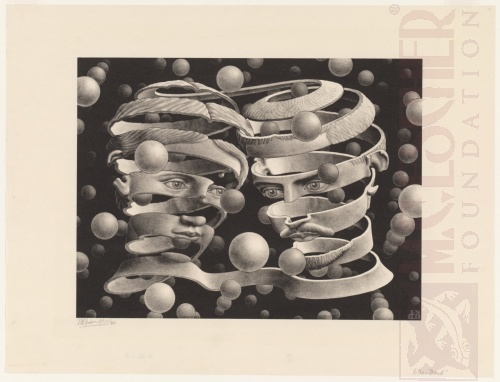
\includegraphics[width=\linewidth]{fig/escher/bound-of-union.jpg}
	\caption{\href{https://mcescher.com/gallery/most-popular/\#iLightbox[gallery\_image\_1]/23}{\emph{Bond of Union}}, M. C. Escher, \textcopyright~The M.C. Escher Company.}
\end{marginfigure}
"Duality" takes its name from the fact that \Cref{prop:containment-hom} can be simply rephrased as
``the preordered set of "conjunctive queries" over $\sigma$ ordered by
"containment" is \emph{dually isomorphic} to the preordered set of "relational databases"
over $\sigma$  order by the homomorphism ordering.'' Symbolically: 
\[
	\tup{\kl[CQ]{\textrm{CQ}_\sigma},\; \contained }
	\isom
	\tup{\kl[relational database]{\textrm{RelDb}_\sigma},\; \cohomto }.
\]
Naturally, to go from "relational databases" to "conjunctive queries",
we associate to any "pointed relational database" $\tup{\?G, \bar g}$
a ""canonical conjunctive query"" $\gamma(\bar g)$ with one atom "atom"
$\+R_{(k)}(x_1,\hdots,x_k)$ for every "hyperedge" $\tup{x_1,\hdots,x_k} \in \+R_{(k)}(\?G)$.
This map is precisely the inverse of the construction defining "canonical databases".

This dual isomorphism has many consequences: essentially every theory that deals with
"relational databases" can be applied to study "conjunctive queries"!

\begin{corollary}[{of "duality" and \Cref{prop:equiv-core-isomorphic}}]
	Two "conjunctive queries" are "semantically equivalent" "iff"
	the "core" of their "canonical database" are "isomorphic".
\end{corollary}

\paragraph*{Graphical depiction of the preordered set of relational databases and conjunctive queries.}
Note that for each "conjunctive query" $\gamma(\bar x)$, the class of
"pointed relational databases" $\tup{\?D, \bar d}$ satisfying the query
is \AP""closed under homomorphisms"", "ie"
\[
	\text{if}\quad \tup{\?D, \bar d} \FOmodels \gamma(\bar x)
	\quad\text{and}\quad \tup{\?D, \bar d} \homto \tup{\?D', \bar d'}
	\quad\text{then}\quad \tup{\?D', \bar d'} \FOmodels \gamma(\bar x).
\]
We represent the preordered set of "relational databases" ordered by $\homto$ as follows:
each equivalence class of "homorphically equivalent" "relational databases" is
represented by a single point. In other words, points are in one-to-one correspondence
with "cores". Then, we represent a point $\core{\?G}$ below another point $\core{\?D}$
whenever $\core{\?G} \homto \core{\?D}$.
For "Boolean queries", this ordering%
\footnote{Formally, from the preordering over "relational databases" we obtained a partial
order over the quotient of "relational databases" by the equivalence class induced by $\homto$,
which happens to be partially ordered set of "cores". Hence, we will interchangeably
use to term \emph{preordering} or \emph{(partial) ordering}.}
admits a unique minimal element, which is the empty database.
For "non-Boolean queries", there is also a minimal "relational database" with
no facts, but that has constants.%
Similarly, there is always a unique maximal element: the "database@@rel" with
a unique vertex $x$ and such that $\+R_{(k)}(x,\dotsc,x)$ holds for
every $\+R_{(k)} \in \sigma$, and all constants are interpreted as this vertex $x$.
We now prove that this poset has a non-trivial structure, assuming that the "signature"
is itself non-trivial.

\begin{proposition}
	\AP\label{prop:poset-reldb}
	Assume that $\sigma$ contains at least one symbol of arity at least 2,
	then the poset of "relational databases"
	admits infinite chains, infinite co-chains and infinite antichains.
\end{proposition}

\begin{proof}
	For the sake of simplicity, we assume that we actually have
	a binary predicate.%
	\footnote{This assumption is "wlog": we can encode the binary 
	relation used in these constructions into any $k$-ary
	relation provided that $k \geq 2$ by encoding $\+E(x,y)$
	as $\+R_{(k)}(x,y,\dotsc,y)$.}

	Clearly, "directed path" provide an infinite chain
	\[
		\pathGraph{1} \homto \pathGraph{2} \homto \cdots
			\homto \pathGraph{n} \homto \pathGraph{n+1} \homto \cdots.
	\]
	We now let $\?C_n$ ($n\in\Np$) denote the directed cycle with domain $\ZnZ{n}$
	and with an edge from $i$ to $j$ "iff" $i+1 = j$.\todo{figure}
	It is then routine to check that for $n,m\in\Np$, we have $\?C_n \homto \?C_m$
	"iff" $n$ is a multiple of $m$. In particular,%
	\footnote{In fact, we obtain a \emph{projective system}. We will discuss
	on projective limits in \todo{ref}.}
	we have
	\[
		\?C_1 \cohomto \?C_2 \cohomto \cdots \cohomto \?C_{2^n} \cohomto \?C_{2^{n+1}} \cohomto \cdots.
	\]
	Finally, $\tup{\?C_p}_{p \text{ prime}}$ is an infinite antichain.
\end{proof}

\begin{figure}
	\centering
	\begin{tikzpicture}[
		font=\footnotesize,
		every node/.style={inner sep=0pt,outer sep=0pt}
	]
		\begin{luacode}
-- parameters to tweak
-- nb of nodes in the lattice
width = 17 -- half-width
height = 17 -- half-height
-- height and width (in cm) of the tikzpicture
display_width = 10
display_height = 10
-- decay rates 
x_opacity_decay = 0.3
y_opacity_decay = 1.5
pos_decay = 1.5

dx = display_width / (2 * width)
dy = display_height / (2 * height)

function grid_to_picture_x(x)
	-- returns the position in the picture from the coordinates in the grid
	return x * dx * (math.abs(x)/width)^(pos_decay-1)
end 
function grid_to_picture_y(y)
	-- returns the position in the picture from the coordinates in the grid
	return y * dy * (math.abs(y)/height)^(pos_decay-1)
end

function is_part_of_grid(x,y)
	in_square = x >= -width and x <= width and y >= -height and y <= height
	in_check = (x+y)%2 ~= 0
	in_diamond = math.abs(x) <= height - math.abs(y)
	return in_square and in_check and in_diamond
end

function is_above(x1,y1,x2,y2) -- check if (x1,y1) is above (x2,y2)
	if y1 < y2 then
		return false
	end
	delta_y = y1 - y2 -- >= 0
	delta_x = math.abs(x2 - x1)
	return (delta_x <= delta_y)
end

function get_color(x,y)
	if y - x == 17 then
		return "c0"
	elseif y + x == -17 then
		return "c2"
	else
		return "black" 
	end
end

function process_opacity(x)
	return (1/(1+math.exp(3.5-20*x)))
end

function get_opacity(x,y)
	if y == 0 then
		return process_opacity(0)
	elseif math.abs(y) == height then
		return process_opacity(1)
	elseif math.abs(y) == 1 and math.abs(x) < width-1 then
		return process_opacity(0.01)
	elseif math.abs(x) == 1 and math.abs(y) < height-1 then
		return process_opacity(0.02)
	elseif math.abs(x) == 0 and math.abs(y) < height-1 then
		return process_opacity(0)
	else
		x_opac = (math.abs(x)/width)^x_opacity_decay
		y_opac = (math.abs(y)/height)^y_opacity_decay
		return process_opacity(x_opac * y_opac)
	end
end

function get_scale(x,y)
	return 2*get_opacity(x,y)^0.3
end

function get_edge_color(x1,y1,x2,y2)
	c1 = get_color(x1,y1)
	c2 = get_color(x2,y2)
	if c1 == c2 then
		return c1
	else 
		return "black"
	end
end

function get_edge_opacity(x1,y1,x2,y2)
	o1 = get_opacity(x1,y1)
	o2 = get_opacity(x2,y2)
	return math.min(o1,o2)
end

-- define coordinates
for x = -width,width do
	for y = -height,height do
		if is_part_of_grid(x,y) then
			tex.print(string.format("\\coordinate (%i %i) at (%.4f, %.4f) {};", x, y, grid_to_picture_x(x), grid_to_picture_y(y)))
		end
	end 
end 
-- draw edges
for x = -width,width do
	for y = -height,height do
		if is_part_of_grid(x,y) then
			above = {{x-1,y+1}, {x+1, y+1}}
			for _, coord in ipairs(above) do 
				x2, y2 = coord[1], coord[2]
				if is_part_of_grid(x2,y2) then
					tex.print(string.format("\\draw[color=%s, opacity=%.4f] (%i %i) to[-] (%i %i);", get_edge_color(x,y,x2,y2), get_edge_opacity(x,y,x2,y2), x, y, x2, y2))
				end
			end
		end
	end 
end 
-- draw grid
for x = -width,width do
	for y = -height,height do
		if is_part_of_grid(x,y) then
			-- white background
			tex.print(string.format("\\node[circle,fill=white, minimum size=%.4f pt] at (%i %i) {};", get_scale(x,y), x, y))
			-- proper colour
			tex.print(string.format("\\node[circle,fill=%s, minimum size=%.4f pt, opacity=%.4f] at (%i %i) {};", get_color(x,y), get_scale(x,y), get_opacity(x,y), x, y))
		end
	end 
end 

\end{luacode}
		\node[above left=2pt of 0 17, color=c0] {$\?C_1$};
		\node[above left=2pt of -1 16, color=c0] {$\?C_2$};
		\node[above left=2pt of -2 15, color=c0] {$\?C_4$};
		\node[above left=2pt of -4 13, color=c0] {\rotatebox{-30}{$\vdots$}};
		\node[above left=2pt of -6 11, color=c0] {$\?C_{2^n}$};
		\node[above left=2pt of -7 10, color=c0] {$\?C_{2^{n+1}}$};
		\node[above left=2pt of -9 8, color=c0] {\rotatebox{-45}{$\vdots$}};

		\node[below left=2pt of 0 -17, color=c2] {$\emptyset$};
		\node[below left=2pt of -1 -16, color=c2] {$\?P_1$};
		\node[below left=2pt of -2 -15, color=c2] {$\?P_2$};
		\node[below left=2pt of -4 -13, color=c2] {\rotatebox{30}{$\vdots$}};
		\node[below left=2pt of -6 -11, color=c2] {$\?P_{n}$};
		\node[below left=2pt of -7 -10, color=c2] {$\?P_{n+1}$};
		\node[below left=2pt of -9 -8, color=c2] {\rotatebox{45}{$\vdots$}};

		\node[circle, fill=white, minimum size=4pt] at (4 -9) {};
		\node[circle, fill=c1, opacity=1, minimum size= 4pt, outer sep=1mm] at (4 -9) {};

		\node[color=c1, align=left, text width=3.8cm, outer sep=1mm] at (3.5, -5) (label-cdb)
			{"\textcolor{c1}{canonical database}@canonical database" $\?G$ of a
			"\textcolor{c1}{Boolean conjunctive query}@Boolean conjunctive query" $\gamma$};
		\draw[draw=c1, semithick] (label-cdb) edge[->,out=90,in=-90] ($(4 -9)+(0, -.1)$);
		\draw[draw=c1, semithick, decorate,decoration={brace,amplitude=5pt,raise=.5em}]
  			(0 17) -- (15 2)
			node[color=c1, midway, above right=5mm, align=left, text width=3.8cm]
				{semantics of $\gamma$};
	\end{tikzpicture}
	\caption{\AP\label{fig:poset-reldb} The poset of "relational databases" over a "signature"
	containing at single binary "predicate", where "homomorphisms" go from bottom to top.
	An infinite chain is represented in red, and an infinite co-chain in blue.
	A large yellow dot represents the "canonical database" of a "conjunctive query",
	while the semantics of this "conjunctive query" is represented with normal-size yellow dots.}
\end{figure}
Based on \Cref{prop:poset-reldb}, we provide an illustration of the ordered set
of "relational databases" in \Cref{fig:poset-reldb}. Notice that, since the semantics
of "conjunctive queries" is closed under "homomorphisms", they are represented by an upper-closed set. Moreover, this set has a unique minimum, corresponding to its "canonical database".
Notice how this representation naturally represents the concept of "duality":
\begin{itemize}
	\item points of the poset ("ie" "relational databases") are in natural
		bijection with upper-closed set that admit a minimum ("ie" "conjunctive queries");
	\item a "conjunctive query" is "contained" in another "iff", by definition,
		the semantics of the former is included in that of the latter, which happens
		"iff" the "canonical database" of the former is above the "canonical database" of the latter
		in \Cref{fig:poset-reldb}.
\end{itemize}

\begin{remark}
	\label{rk:database-vs-structures}
	À propos "relational databases" "vs" "relational structures",
	these posets are actually isomorphic 
	since a "relational structure" is always "homomorphically equivalent"
	to the structure in which we removed "isolated vertices".
\end{remark}

\paragraph*{The Distributive Lattice of Relational Databases}

\Cref{prop:poset-reldb} shows that the poset of "relational databases" has a somewhat
complex structure, in the sense that it is infinite height, co-height and width.
However, we next show that it has a rich algebraic structure.

\begin{marginfigure}
	\centering
	\begin{tikzcd}[row sep=huge]
		\tup{\?D_1,\bar d_1} &[-4em] &[-4em] \tup{\?D_2,\bar d_2} \\ 
		& \tup{\?D_1,\bar d_1} \prodstruct \tup{\?D_2,\bar d_2}
			\ar[ul, "\projHom{1}" swap] \ar[ur, "\projHom{2}"]
		& \\
		& \tup{\?U, \bar u} \ar[u, "g", dashed]
			\ar[uul, "f_1", bend left] \ar[uur, "f_2" swap, bend right]
		&
	\end{tikzcd}
	\caption{\AP\label{fig:cartesian-product-diagram} Universal property satisfied
	by the "Cartesian product".}
\end{marginfigure}
In light of \Cref{rk:database-vs-structures}, the "Cartesian product"
of two "relational databases" $\tup{\?D_1,\bar d_1}$ and $\tup{\?D_2,\bar d_2}$
whose tuples have the same arity
is well-defined: we consider their product $\tup{\?D_1,\bar d_1} \prodstruct \tup{\?D_2,\bar d_2}$
as "relational structures", and remove all "isolated vertices".
We slightly abuse the notation and still denote this product by $\reintro{\prodstruct}$.
It is routine to check that this "Cartesian product" in indeed a Cartesian product in
the categorical sense, "ie" that it satisfies the universal property
that first it has "homomorphisms" $\projHom{1}$ and $\projHom{2}$ to both $\tup{\?D_1,\bar d_1}$ and $\tup{\?D_2,\bar d_2}$, and that moreover it is the smallest object satisfying this property,
in the sense that for every "relational database" $\tup{\?U, \bar u}$ with "homomorphisms"
$f_1$ and $f_2$ to $\tup{\?D_1,\bar d_1}$ and $\tup{\?D_2,\bar d_2}$, 
then there exists a unique "homomorphism" $g$ from $\tup{\?U, \bar}$ to
$\tup{\?D_1,\bar d_1}$ and $\tup{\?D_2,\bar d_2}$ such that
the diagram of \Cref{fig:cartesian-product-diagram} commutes:
this "homomorphism" $g$ is actually $f_1 \times f_2\colon u \mapsto \tup{f_1(u), f_2(u)}$.
Going back to the poset structure, this implies that any pair of points must have an infimum.
\begin{fact}
	Given two finite "relational databases", their "Cartesian product"
	is their greatest lower bound in the poset of "relational databases"
	ordered by $\homto$.
\end{fact}

Similarly, the "disjoint union" satisfies the property dual to \Cref{fig:cartesian-product-diagram}.
\begin{fact}
	Given two finite "relational databases", their "disjoint union"
	is their least upper bound in the poset of "relational databases"
	ordered by $\homto$.
\end{fact}

Put together, these facts imply that the poset of "relational databases" is
actually a bounded lattice! It is moreover distributive
since the isomorphism
\[
	\?A \prodstruct (\?B \disunion \?C) \isom (\?A \prodstruct \?B) \disunion (\?A \prodstruct \?C)
\]
holds for any "databases@@rel" $\?A$, $\?B$ and $\?C$.
But then, by "duality", we get that the poset of "conjunctive queries"
under "containment" is also a "distributive lattice"!
We shall see that the greatest lower bound and least upper bound
have a natural logical interpretation, and that moreover
this structure of "distributive lattice" will help us
deal with "CQs": in particular, it will be at the heart of
solving the "synthesis problem". 


\paragraph*{The Distributive Lattice of Conjunctive Queries.}

Given two "CQs" $\gamma(\bar x)$ and $\delta(\bar y)$,
where $\bar x$ and $\bar y$ have the same arity, we define
its \AP""disjoint conjunction"", denoted by
$\gamma(\bar x) \intro*\disconj \delta(\bar y)$,
to be the "CQs" obtained by taking the "disjoint union" of "atoms" 
of the "CQs" and then identifying the elements of $\bar x$ and $\bar y$ pointwise.
For instance, letting $\gamma(x) \defeq x \atom{a} y$ be the query
asking for all elements with an outgoing $a$-edge,
and $\delta(x) \defeq x \atom{b} y$ be the query
asking for all elements with an outgoing $a$-edge,
then their "disjoint conjunction" $\gamma(x) \disconj \delta(x)$ is
\[
	\alpha(x) \defeq x \atom{a} y \land x \atom{b} y'
\]
and outputs all elements with both an outgoing $a$-edge and an outgoing $b$-edge.%
\footnote{As for "disjoint union", the name "disjoint conjunction" is slightly abusive
but justified by its universal property.}

\begin{fact}
	The "canonical database" of the "disjoint conjunction"
	equals the "disjoint union" of the "canonical databases".
	By "duality", it follows that
	the "disjoint conjunction" is the greatest lower bound
	of two "CQs".%
	\footnote{Careful: "duality" is precisely a \emph{dual} isomorphism,
	"ie" it reverses the order. Hence, a least upper bound ("disjoint union")
	becomes a greatest lower bound ("disjoint conjunction").}
\end{fact}

The other operator (the dual of "Cartesian product")
does not have such a nice intuitive interpretation---however
it does not mean that it will be less useful, on the contrary!
While "conjunctive queries" are not closed under
union---we will see this in \todo{ref}---, this operator
acts as the best approximation of it.

\begin{definition}
	We define the \AP""weak union"" \AP$\intro*\weakunion$ of two "CQs"
	with the same number of "output variables"
	as the "canonical CQ" of the "Cartesian produt" of their "canonical databases".
\end{definition}

By construction, it is their greatest upper bound,
in the sense that
$\gamma(\bar x) \contained \gamma(\bar x) \weakunion \delta(\bar y)$,
$\delta(\bar y) \contained \gamma(\bar x) \weakunion \delta(\bar y)$,
and $\gamma(\bar x) \weakunion \delta(\bar y)$ is the smallest "CQ" satisfying this property.

For instance, if $\gamma() \defeq x \atom{a} y$ asks for the existence of an $a$-edge
and $\delta() \defeq x \atom{b} y$, then $\gamma() \weakunion \delta()$ is the empty "CQ",
"ie" the "CQ" that always true: knowing that a "database" contains either an $a$-edge
or a $b$-edge is as good as knowing nothing in terms of "CQ" expressivity.
On the other hand, if $\gamma(x) \defeq x \atom{a} y \atom{b} z$ asks the source of all 
$ac$-paths and $\delta(x) \defeq a \atom{b} y \atom{c} z$ asks for the source of all $bc$-paths,
then $\gamma(x) \weakunion \delta(x)$ will be "homomorphically equivalent" to
$\alpha(x) \defeq x \atom{a} y$ which outputs all sources of $a$-edges.

We summarized the properties of the two distributive lattices
in \Cref{tab:distributive-lattices}. Note that, all notions
occurring in this table, be it the orders or the binary operators,
require the "CQs" to the same number of "output variables",
and the (pointed) "relational databases" to have tuples of the same size,
and so in fact we obtain two lattices for every possible arity/tuple size.
This also motivates the somewhat counter-intuitive definition of the
"disjoint union" for "structures" over "signatures" that are not
"purely relational@@signature".

\begin{table}
	\centering
	\begin{tabular}{ccc}
		\toprule
		 & "Conjunctive Queries" & "Relational Databases" \\ \midrule
		\multirow{2}{*}{preorder} & \multirow{2}{*}{"containment" $\contained$} & existence of\\
		& & "homomorphisms" $\homto$ \\
		least upper bound & "weak union" $\weakunion$ & "disjoint union" $\disunion$ \\
		greatest lower bound & "disjoint conjunction" $\disconj$ & "Cartesian product" $\prodstruct$ \\ 
		\multirow{2}{*}{greatest element} & \multirow{2}{*}{``true'' (empty "CQ")} & single vertex \\
		& & will all "hyperedges" \\
		\multirow{2}{*}{least element} & single variable & \multirow{2}{*}{empty "database@@rel"}
		\\
		& will all "hyperedges" & \\ \bottomrule
	\end{tabular}
	\caption{
		\AP\label{tab:distributive-lattices}
		The distributive lattices of "conjunctive queries" and "relational databases".
		By "duality", one can go from one lattice to the \emph{opposite} of the other
		by taking "canonical databases" or "canonical conjunctive queries".}
\end{table}

Amongst bounded distributive lattices, the better behaved are
the Boolean algebras, in which every element has a complement.
In our case, this would be an operator $\neg$ "st" for every "database@@rel" $\?D$,
then $\?D \prodstruct {\neg \?D}$ would be "homomorphically equivalent" to
the empty database and $\?D \disunion {\neg \?D}$ to the greatest database,
"ie" consisting of a single vertex and all possible "hyperedges" over it.

\begin{proposition}
	The distributive lattice of "databases@@rel" (and hence of
	"conjunctive queries") does not admit complementation.
\end{proposition}

\begin{proof}
	Assume that the "signature" is non-trivial and let $\?D$ be a non-trivial "database@@rel",
	"ie" neither the least nor greatest element of the lattice.
	To ensure that $\?D \disunion {\neg \?D}$ is "homomorphical equivalent"
	to the greatest database, $\neg \?D$ must actually be "homomorphical equivalent" to 
	the greatest database itself,
	but then $\?D \prodstruct {\neg \?D}$ would be non-empty.
\end{proof}

However, "conjunctive queries" still have a bit more structure: we shall
see that they are a Heyting algebra, namely that it is a bounded distributive lattice
with the extra property that for every $\gamma(\bar x)$ and $\delta(\bar y)$,
where $\bar x$ and $\bar y$ have the same arity, then there exists
a greatest element $\chi(\bar z)$ "st"
\[
	\gamma(\bar x) \disconj \chi(\bar z) \contained \delta(\Bar z). 
\]
This greatest element $\chi(\bar z)$ is denoted by $\gamma(\bar x) \impH \delta(\bar y)$, and is called \emph{implication}.%
\footnote{Heyting algebras were introduced to model intuitionistic logic.
It is not hard to see that the implication $\phi \Rightarrow \psi$
does satisfy the property it is the greatest formula $\chi$
"st" $\psi \land \chi$ entails $\psi$.}

\begin{proposition}
	\!\footnote{The fact that "conjunctive queries" and "conjunctive queries" form
	a bounded distributive lattice is folklore.}
	The bounded distributive lattice of "conjunctive queries" is actually
	a Heyting algebra.
\end{proposition}

\begin{proof}
	We use "duality" to prove this and in fact
	rather prove that "relational databases" form a ``co-Heyting algebra'',
	in the sense that for any "databases" $\tup{\?G, \bar g}$ and $\tup{\?D, \bar d}$,
	there exists a least element $\tup{\?X, \bar x}$ "st"
	\[
		\tup{\?G, \bar g} \disunion \tup{\?X, \bar x} \cohomto \tup{\?D, \bar d}:
	\]
	$\tup{\?X, \bar x}$ is actually obtained by taking the "disjoint union"
	of all "connected components" of $\tup{\?D, \bar d}$ 
	that cannot be "mapped homomorphically" to $\tup{\?G, \bar g}$.
	The operator $\impH$ can then be explicitly constructed by "duality".
\end{proof}

By construction of $\impH$, it comes naturally equipped with some
form of Currying, in the sense that
\[
	\tup{\?A, \bar a}
	\FOmodels \gamma(\bar x) \impH \delta(\bar y)
	\quad\text{"iff"}\quad
	\tup{\?A, \bar a} \disunion \tup{\?G, \bar x}
	\FOmodels \delta(\bar y),
\]
for any "CQs" $\gamma(\bar x)$ and $\delta(\bar y)$
and any "relational database" $\tup{\?A, \bar a}$,
where $\tup{\?G, \bar x}$ denotes the "canonical database" of $\gamma(\bar x)$.
Similarly, as expected, we have
\[
	\gamma(\bar x) \disconj (\gamma(\bar x) \impH \delta(\bar y))
	\semequiv
	\delta(\bar y).
\]


\begin{itemize}
	\item combined complexity / data Complexity
	\itemAP $\intro*\underlying{\gamma}$ and ""underlying graph""
	\itemAP ""equality atom""
	\itemAP ""evaluation map@@cq"" (explain why notion is necessary by pointing to "evaluation map" for CRPQs)
	\itemAP ""disjunct""
\end{itemize}

\subsection{Static Analysis of Conjunctive Queries}

\subsection{Intermezzo: Parametrized Complexity Classes}

\begin{itemize}
	\itemAP ""FPT""
	\itemAP ""W1""
	\itemAP ""XP""
\end{itemize}

\subsection{Beyond Conjunctive Queries}